\begin{mainquestion}{csvtcquadratic}{Does Solving The Quadratic Equation Really Matter?}

\questionpoints
In this problem we will see if we can take some short-cuts when we compute the DC voltage transfer characteristic of an amplifier. Consider an NMOS common-source amplifier with a resistive load $R_D = 14 \text{ k}\Omega$ connected to a supply voltage $V_{DD} = 10 \text{ V}$. The transistor parameters are threshold voltage $V_{tn} = 1 \text{ V}$ and transconductance parameter $k_n = 1.0 \text{ mA/V}^2$. Channel-length modulation can be neglected ($\lambda = 0$). Assume the input voltage ranges from 0-5V.

\begin{center}
\begin{circuitikz}[american]
    \draw (0,0) node[nmos] (Q1) {};
    \draw (Q1.S) node[ground] {};
    \draw (Q1.G) to[short, -o] (-1.5, 0) node[left] {$v_I$};
    \draw (Q1.D) to[short, *-o] (1.5, 0.76) node[right] {$v_O$};
    \draw (Q1.D) to[R, l_=$14 \text{ k}\Omega$] (0, 3) node[vcc] {$10 \text{ V}$};
\end{circuitikz}
\end{center}

\renewcommand{\labelenumi}{(\alph{enumi})}

% =========================================================
\begin{partquestion}{saturationvtc}
{Derive the piecewise expression for the Voltage Transfer Characteristic (i.e., $v_O$ as a function of $v_I$) using the Shichman-Hodges (square-law) equations. For this part, ignore the fact that the transistor enters the triode region, and have the saturation region stop when the output voltage = 1V. Clearly define the numerical ranges of $v_I$ for the cutoff region and this ``pseudo saturation" region.

\textit{Hint: A generic version of this derivation is covered in Lecture 15.}}

\begin{answer}[3.5in]
        \textbf{Cutoff:} For $v_I < 1 \text{ V}$, the transistor is off, so $i_D = 0 \text{ mA}$. \\
        Therefore, there is no voltage drop across $R_D$, and $v_O = 10 \text{ V}$. \\
        
        \textbf{Pseudo-Saturation:} The transistor is in saturation. \\
        The current is $i_D = \frac{1}{2} k_n (v_I - V_{tn})^2 = \frac{1}{2}(1.0)(v_I - 1)^2 \text{ mA}$. \\
        The output voltage is $v_O = V_{DD} - i_D R_D = 10 - \left[ \frac{1}{2}(1.0)(v_I - 1)^2 \right] \times 14$. \\
        Simplifying: $v_O = 10 - 7(v_I - 1)^2 \text{ V}$. \\
        
        To find the numerical range, we are told to stop when $v_O = 1 \text{ V}$: \\
        $1 = 10 - 7(v_I - 1)^2 \implies 7(v_I - 1)^2 = 9 \implies (v_I - 1) = \sqrt{\frac{9}{7}} \approx 1.134 \text{ V}$. \\
        $v_I = 1 + 1.134 = 2.134 \text{ V}$. \\
        Thus, this pseudo-saturation region is valid for $1 \text{ V} \leq v_I \leq 2.134 \text{ V}$.
\end{answer}

\qnewpage
\end{partquestion}

% =========================================================
\begin{partquestion}{trioderegion}
{Now, let's tackle when the transistor is in the triode region.  In this part, you will compute the ``right" answer.  Using the nMOS current equation in the triode region, compute the $v_I$ when the circuit enters this region and the resulting output voltage $v_O$.  To generate the answer requires solving a quadratic equation.}

\begin{answer}[3in]
        \textbf{Triode Entry Point:} The transition from saturation to triode occurs when $v_O = v_I - V_{tn} = v_I - 1$. \\
        Substituting $v_I - 1 = v_O$ into the saturation equation: $v_O = 10 - 7v_O^2$. \\
        Rearranging: $7v_O^2 + v_O - 10 = 0$. \\
        Using the quadratic formula: $v_O = \frac{-1 + \sqrt{1^2 - 4(7)(-10)}}{2(7)} = \frac{-1 + \sqrt{281}}{14} \approx 1.126 \text{ V}$. \\
        The corresponding input voltage is $v_I = v_O + 1 \approx 2.126 \text{ V}$. \\
        
        \textbf{Triode Region ($v_I > 2.126 \text{ V}$):} \\
        The current is $i_D = k_n \left[ (v_I - V_{tn})v_O - \frac{1}{2}v_O^2 \right] = 1.0 \left[ (v_I - 1)v_O - \frac{1}{2}v_O^2 \right] \text{ mA}$. \\
        The output voltage is $v_O = 10 - 14 \left[ (v_I - 1)v_O - \frac{1}{2}v_O^2 \right] \text{ V}$. \\
        Rearranging into a standard quadratic: $7v_O^2 - (14(v_I - 1) + 1)v_O + 10 = 0$. \\
        Solving for $v_O$ provides the rigorous triode curve: \\
        $v_O = \frac{14(v_I - 1) + 1 - \sqrt{(14(v_I - 1) + 1)^2 - 280}}{14} \text{ V}$.
\end{answer}

\end{partquestion}

% =========================================================
\begin{partquestion}{triodelinear}
{Let's solve for the triode region again, but this time we will use the linear model of the transistor (which is true for small $V_{DS}$) by ignoring how the current bends over at higher $V_{DS}$.  Using this linear model, how does the output voltage $v_O$ vary with $v_I$?}

\begin{answer}[2in]
        Using the deep triode (linear) model for small $V_{DS}$: 
        \[i_D \approx k_n (v_I - V_{tn})v_O = 1.0(v_I - 1)v_O \frac{\text{ mA}}{V^2} \implies R_T=\frac{1}{1.0(v_I - 1)}k\Omega\]. \\
        where $R_T$ is the effective resistance of the transistor. Using the voltage divider equation gives:
        \[v_O=\frac{R_T}{R_T+R_D}10V= \frac{\frac{k\Omega}{1.0(v_I - 1)}}{\frac{k\Omega}{1.0(v_I - 1)}+14K\Omega}10V=\frac{10V}{(1+14(v_I - 1))}\]
        You could also solve it by equating the currents. The output voltage is:\\
        $v_O = V_{DD} - i_{DS} R_D = 10 - 14(v_I - 1)v_O.$ 
        Rearranging to solve for $v_O$: \\
        $v_O + 14(v_I - 1)v_O = 10$ \\
        $v_O (1 + 14(v_I - 1)) = 10$ \\
        $v_O = \frac{10}{1 + 14(v_I - 1)} \text{ V}$. \\
        This shows $v_O$ varies inversely with $(v_I - 1)$ in the linear approximation.
\end{answer}

\qnewpage
\end{partquestion}

% =========================================================
\begin{partquestion}{plotvtc}
{Plot the rigorous VTC from Part (a) and (b) and the approximated VTC from Part (a) and (c) on the same axes. You may use any graphing software of your choice. Does the simpler model provide a reasonable approximation of the VTC?}

\begin{answer}[3.5in]
        \begin{center}
        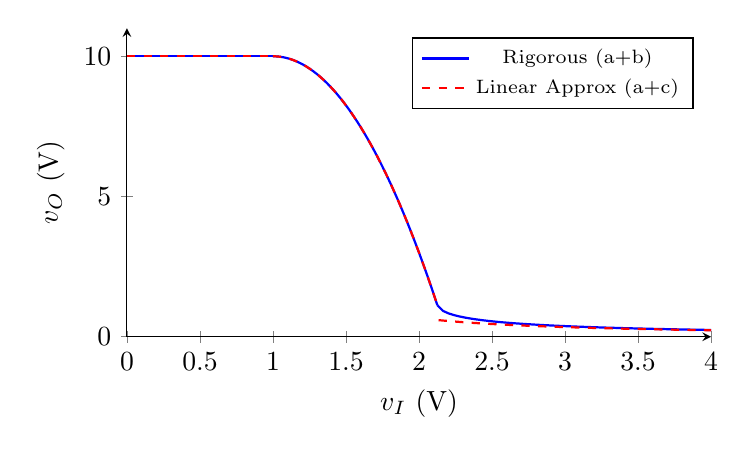
\begin{tikzpicture}
        \begin{axis}[
            width=9cm, height=5.5cm,
            axis lines = left,
            xlabel = {$v_I$ (V)}, ylabel = {$v_O$ (V)},
            ymin=0, ymax=11, xmin=0, xmax=4,
            legend pos=north east,
            legend style={font=\scriptsize}
        ]
        % Rigorous Model (Part a + b)
        \addplot [domain=0:1, samples=2, thick, blue] {10};
        \addlegendentry{Rigorous (a+b)}
        \addplot [domain=1:2.126, samples=50, thick, blue, forget plot] {10 - 7*(x-1)^2};
        \addplot [domain=2.126:4, samples=50, thick, blue, forget plot] { (1 + 14*(x-1) - sqrt((1 + 14*(x-1))^2 - 280)) / 14 };
        
        % Linear Approx. Model (Part a + c) 
        \addplot [domain=0:1, samples=2, thick, dashed, red] {10};
        \addlegendentry{Linear Approx (a+c)}
        \addplot [domain=1:2.134, samples=50, thick, dashed, red, forget plot] {10 - 7*(x-1)^2};
        \addplot [domain=2.134:4, samples=50, thick, dashed, red, forget plot] { 10 / (1 + 14*(x-1)) };
        \end{axis}
        \end{tikzpicture}
        \end{center}
        
        Note. discontinuities in the graph are acceptable given the ``psudo-sautration" range defined in part a.
        
        \textbf{How good is this model?} \\
        The simple approximation (a+c) matches perfectly in saturation but creates a massive discontinuity (a sudden jump) when entering the triode region. This shows that the deep-triode equation is a poor approximation for the transition region, as it assumes the transistor immediately drops to a low resistance. 
\end{answer}

\end{partquestion}

% =========================================================
\begin{partquestion}{linearmodel}
{An even simpler model would be to create a linear model of the amplifier by just measuring the gain around one operating point. Calculate the small-signal voltage gain $A_v = \frac{dv_O}{dv_I}$ at a DC bias of $V_I = 1.5 \text{ V}$. Assume the output follows that line until it hits the power supply or ground. Add this small-signal tangent line to your plot in part (d). How good is this small-signal model?}

\begin{answer}[3in]
    \begin{center}
        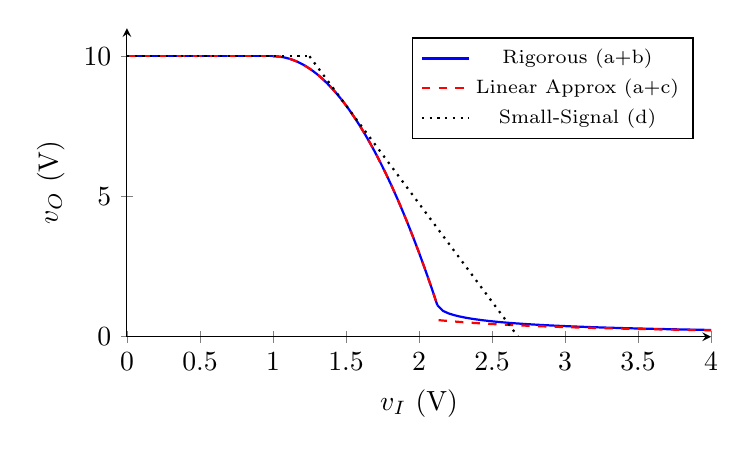
\begin{tikzpicture}
        \begin{axis}[
            width=9cm, height=5.5cm,
            axis lines = left,
            xlabel = {$v_I$ (V)}, ylabel = {$v_O$ (V)},
            ymin=0, ymax=11, xmin=0, xmax=4,
            legend pos=north east,
            legend style={font=\scriptsize}
        ]
        % Rigorous Model (Part a + b)
        \addplot [domain=0:1, samples=2, thick, blue] {10};
        \addlegendentry{Rigorous (a+b)}
        \addplot [domain=1:2.126, samples=50, thick, blue, forget plot] {10 - 7*(x-1)^2};
        \addplot [domain=2.126:4, samples=50, thick, blue, forget plot] { (1 + 14*(x-1) - sqrt((1 + 14*(x-1))^2 - 280)) / 14 };
        
        % Linear Approx. Model (Part a + c) 
        % Transitions at v_I = 2.134V based on Part (a) limits
        \addplot [domain=0:1, samples=2, thick, dashed, red] {10};
        \addlegendentry{Linear Approx (a+c)}
        \addplot [domain=1:2.134, samples=50, thick, dashed, red, forget plot] {10 - 7*(x-1)^2};
        \addplot [domain=2.134:4, samples=50, thick, dashed, red, forget plot] { 10 / (1 + 14*(x-1)) };

        % Small-Signal Tangent Model (from part d)
        \addplot [domain=0:1.25, samples=2, thick, dotted, black] {10};
        \addlegendentry{Small-Signal (d)}
        \addplot [domain=1.25:2.678, samples=2, thick, dotted, black, forget plot] {18.75 - 7*x};
        \addplot [domain=2.678:4, samples=2, thick, dotted, black, forget plot] {0};
        \end{axis}
        \end{tikzpicture}
        \end{center}
        
        \textbf{Small-Signal Linear Model at $V_I = 1.5\text{ V}$:} \\
        At $V_I = 1.5\text{ V}$, the transistor is in saturation. The DC output voltage is: \\
        $V_O = 10 - 7(1.5 - 1)^2 = 10 - 7(0.25) = 8.25 \text{ V}$. \\
        Taking the derivative of the saturation equation: $A_v = \frac{dv_O}{dv_I} = -14(v_I - 1)$. \\
        At $v_I = 1.5\text{ V}$, the small-signal gain is $A_v = -14(0.5) = \mathbf{-7 \text{ V/V}}$. \\
        
        The equation for this tangent line model is: \\
        $v_O = V_O + A_v(v_I - V_I) = 8.25 - 7(v_I - 1.5) = 18.75 - 7v_I \text{ V}$. \\
        Following this line, it hits $10 \text{ V}$ at $v_I \approx 1.25 \text{ V}$ and $0 \text{ V}$ at $v_I \approx 2.68 \text{ V}$. \\
        
        \textbf{How good is this model?} \\
        The small-signal tangent line model is an excellent approximation for \textbf{small signal excursions} directly around the $V_I = 1.5 \text{ V}$ operating point. However, it is a poor model for the overall VTC because it completely ignores the non-linear, quadratic nature of the saturation region and fails to capture the abrupt transitions into the cutoff and triode regions.
\end{answer}

\end{partquestion}

\end{mainquestion}
